\subsubsection{Size changes}

Flow through contractions/expansions cause the flow to accelerate/decelerate so it is important to consider size changes when pipes of different diameter are connected. Contractions and expansions are really two sides of the same coin, a contraction with flow in the opposite direction is an expansion just as an expansion with reverse flow is a contraction. Lets consider contractions and expansions separately before their action with reverse flow and combining them into a single component.  

\paragraph{Contraction}

Let us consider a contraction where the flow is from inlet node $i$ to outlet node $k$, as shown in figure \ref{fig:contraction_diagram}. The head loss due to the contraction \cite{rennels22} is given by
\begin{align}
H_L = \frac{K_c V_i^2}{2g},
\end{align}
where the contraction loss coefficient is
\begin{align*}
K_c = 0.0696 \left( 1 - \beta^2 \right) \lambda^2 + \left( \lambda - 1 \right)^2
\end{align*}
and
\begin{align*}
\lambda = 1 + 0.622 \left( 1 - 0.215 \beta^2 - 0.785 \beta^5 \right).
\end{align*}
Here $\beta = d_k / d_i$ is the ratio of the smaller diameter to the larger diameter and $V_i = Q_j / A_i$ is the inlet flow velocity. 

\begin{figure}
\centering
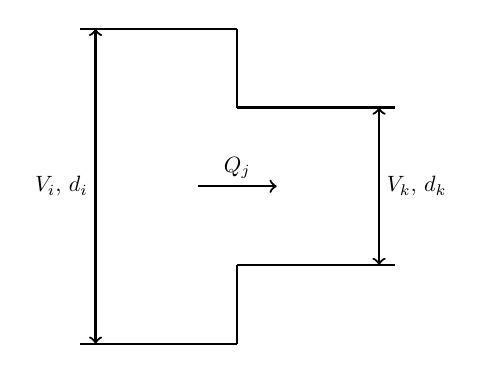
\begin{tikzpicture}[ scale=1, every node/.style={scale=0.8},] 
% Inlet pipe
\draw[thick] (0,0) -- (-2,0);
\draw[thick] (0,4) -- (-2,4);
% Contraction
\draw[thick] (0,0) -- (0,1);
\draw[thick] (0,4) -- (0,3);
% Outlet pipe
\draw[thick] (0,1) -- (2,1);
\draw[thick] (0,3) -- (2,3);
% Annotations
\node[anchor=east] at (-1.8,2) {$V_i$, $d_i$};
\draw[thick, <->] (-1.8,0) -- (-1.8,4);
\node[anchor=south] at (0,2) {$Q_j$};
\draw[thick, ->] (-0.5,2) -- (0.5,2);
\node[anchor=west] at (1.8,2) {$V_k$, $d_k$};
\draw[thick, <->] (1.8,1) -- (1.8,3);
\end{tikzpicture} 
\caption{An abrupt contraction where positive flow is from $i$ to $k$. The size ratio is $\beta = d_k / d_i$.}
\label{fig:contraction_diagram}
\end{figure}

\paragraph{Expansion}

For an expansion where the flow is from inlet node $i$ to outlet node $k$, as shown in figure \ref{fig:expansion_diagram} the head loss due to the expansion \cite{rennels22} is given by
\begin{align}
H_L = \frac{\hat{K}_e V_i^2}{2g},
\end{align}
where
\begin{align*}
\hat{K}_e = \left(1 - \hat{\beta}^2 \right)^2
\end{align*}
and $\hat{\beta} =  d_i / d_k$.

\begin{figure}
\centering
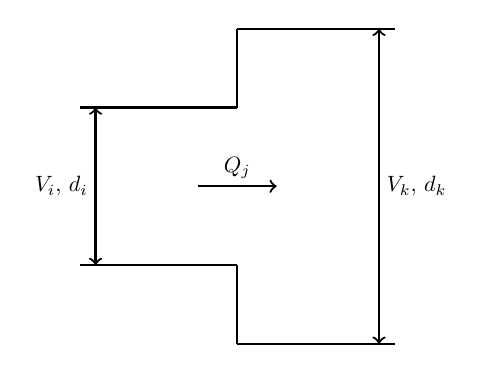
\begin{tikzpicture}[ scale=1, every node/.style={scale=0.8},] 
% Outlet pipe
\draw[thick] (0,0) -- (2,0);
\draw[thick] (0,4) -- (2,4);
% Contraction
\draw[thick] (0,0) -- (0,1);
\draw[thick] (0,4) -- (0,3);
% Inlet pipe
\draw[thick] (0,1) -- (-2,1);
\draw[thick] (0,3) -- (-2,3);
% Annotations
\node[anchor=west] at (1.8,2) {$V_k$, $d_k$};
\draw[thick, <->] (1.8,0) -- (1.8,4);
\node[anchor=south] at (0,2) {$Q_j$};
\draw[thick, ->] (-0.5,2) -- (0.5,2);
\node[anchor=east] at (-1.8,2) {$V_i$, $d_i$};
\draw[thick, <->] (-1.8,1) -- (-1.8,3);
\end{tikzpicture} 
\caption{An abrupt expansion where positive flow is from $i$ to $k$. The size ratio is $\hat{\beta} = d_i / d_k$.}
\label{fig:expansion_diagram}
\end{figure}

\paragraph{Reverse flow}

For positive flows, $Q_j > 0$, if $\beta < 1$ or $\hat{\beta} > 1$ then we have a contraction but if $\beta > 1$ or $\hat{\beta} < 1$ then we have an expansion. For negative flows, $Q_j < 0$, the situation is reversed if $\beta < 1$ or $\hat{\beta} > 1$ then we have an expansion but if $\beta > 1$ or $\hat{\beta} < 1$ then we have a contraction.

Reverse flow in a contraction, see figure \ref{fig:contraction_diagram}, is actually an expansion with a head loss given by
\begin{align}
H_L = \frac{K_e V_k^2}{2g},
\end{align}
where
\begin{align*}
K_e = \left(1 - \beta^2 \right)^2.
\end{align*}

Similarly reverse flow in an expansion, see figure \ref{fig:expansion_diagram}, is actually a contraction with a head loss given by
\begin{align}
H_L = \frac{\hat{K}_c V_k^2}{2g},
\end{align}
where 
\begin{align*}
\hat{K}_c = 0.0696 \left( 1 - \hat{\beta}^2 \right) \hat{\lambda}^2 + \left( \hat{\lambda} - 1 \right)^2
\end{align*}
and
\begin{align*}
\hat{\lambda} = 1 + 0.622 \left( 1 - 0.215 \hat{\beta}^2 - 0.785 \hat{\beta}^5 \right).
\end{align*}

\paragraph{Resistance for abrupt size changes}

These four different scenarios for forward/reverse flow and $\beta = \hat{\beta}^{-1}$ greater/less than $1$ means the resistance term for an abrupt size changes must be split into four parts. 
\begin{align}\label{abrupt_size_change_resistance}
\boxed{
  \!\begin{gathered}
  R_j = -\frac{K Q_j^2}{2 A} + g A \Delta H_j, \hspace{0.5cm} \text{where} \\
A = \begin{cases}
A_i &\text{if} \hspace{0.5cm} Q_j > 0,\\
A_k &\text{if} \hspace{0.5cm} Q_j < 0,
\end{cases} \nonumber \\
K = \begin{cases} 
K_c, &\text{if} \hspace{0.5cm} Q_j > 0, \beta < 1, \\
\hat{K}_e, &\text{if} \hspace{0.5cm} Q_j > 0, \beta > 1, \\
K_e, &\text{if} \hspace{0.5cm} Q_j < 0, \beta < 1, \\
\hat{K}_c, &\text{if} \hspace{0.5cm} Q_j < 0, \beta > 1.
\end{cases} \nonumber
  \end{gathered}
}
\end{align}